\subsection{Двумерный датасет, количество классов 5}
Датасет был сгенерирован с помощью функции \textit{make\_blobs} библиотеки \textbf{sklearn}. Пример использования можно посмотреть в директории code/dataset\_generator.py. Входные параметры:
\begin{enumerate}
	\item -{}-n\_samples (значение по умолчанию 1000) "--- количество примеров;
	\item -{}-n\_features (значение по умолчанию 2) "--- количество признаков;
	\item -{}-classes (значение по умолчанию 5) "--- количество классов;
	\item -{}-shuffle (значение по умолчанию \textit{true}) "--- нужно ли перетасовать примеры;
	\item -{}-random\_state (значение по умолчанию 42) "--- seed для генерации.
\end{enumerate}
Результат генерации со значениями по умолчанию приведён на рис. \ref{img:blobs}.
\begin{figure}[h]
	\centering
	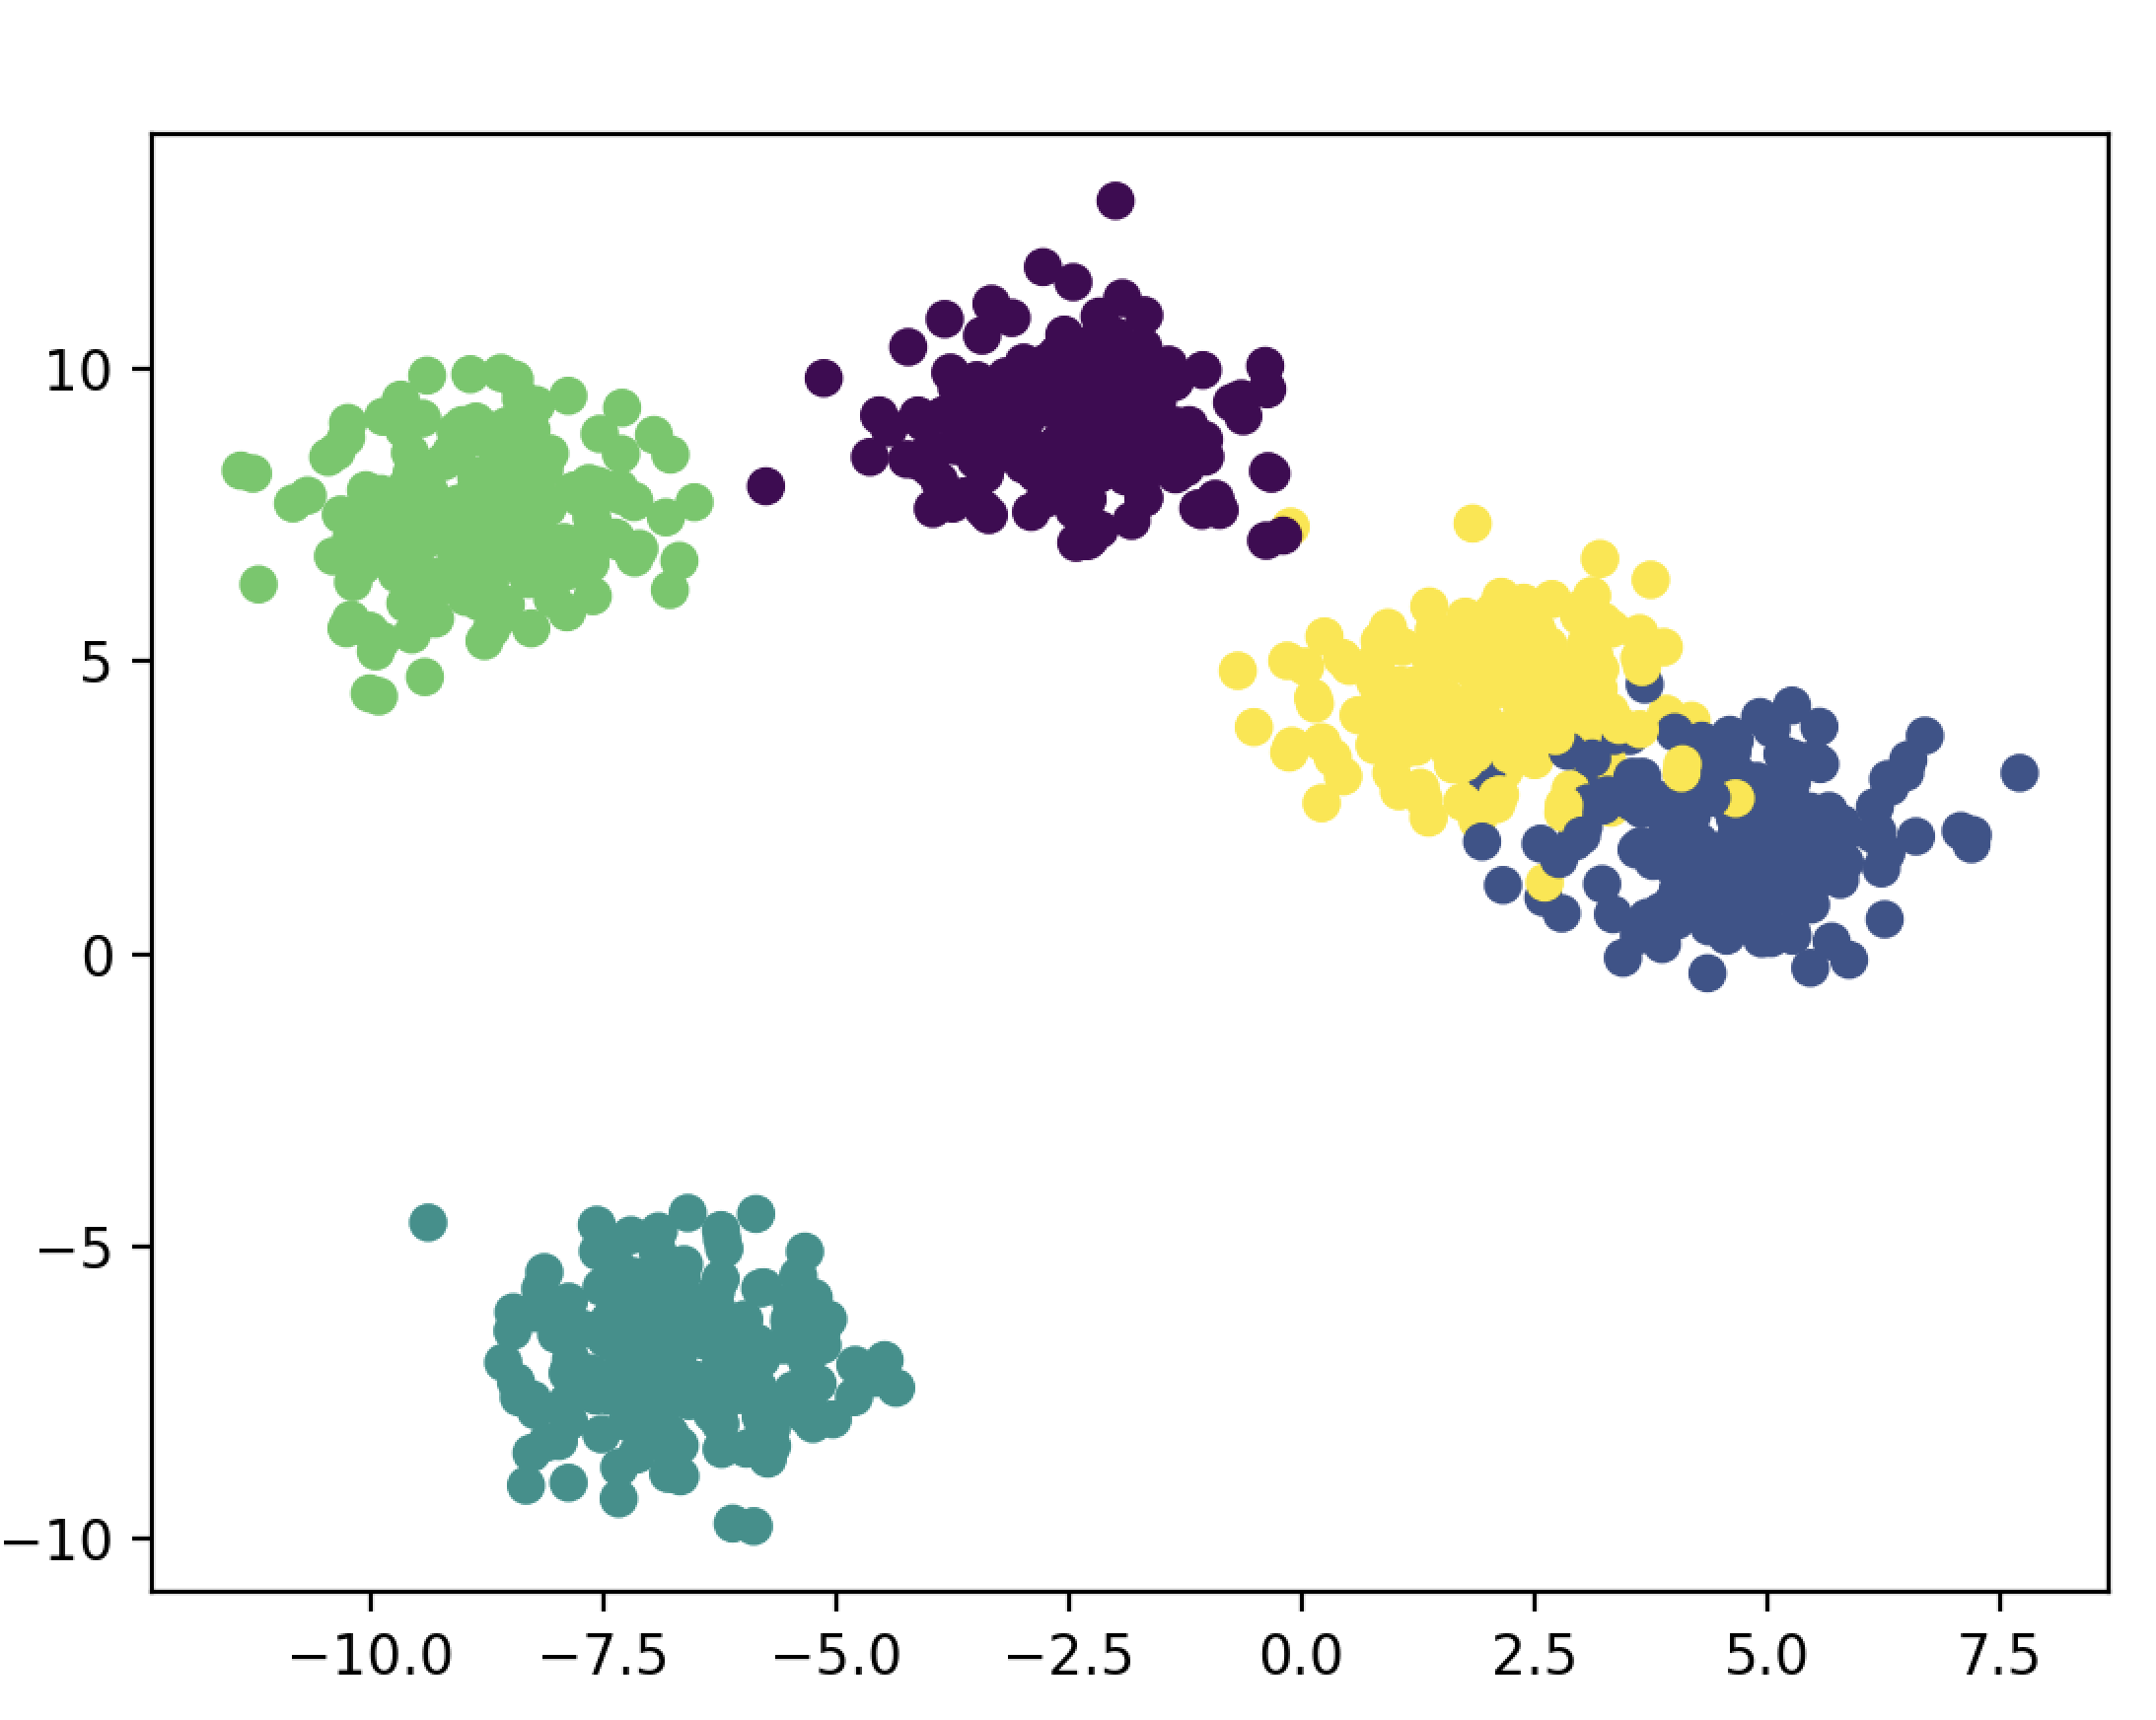
\includegraphics[width=0.8\linewidth]{images/blobs}
	\caption{Сгенерированный набор данных}
	\label{img:blobs}
\end{figure}

Алгоритм работы кода в \textit{code/main.py}:
\begin{enumerate}
	\item Создаётся по экзмпляру класса Perceptron и SGDClassifier;
	\item Считывается датасет из файла \textit{generated\_dataset.csv};
	\item Запускается обучение модели;
	\item Рисуется \textit{Decision surface};
	\item Рисуется набор данных;
	\item В консоль выводятся метрики, достигнутые на тестовой выборке.
\end{enumerate}

Следующие результаты были получены при инициализации класса перцептрона и линейного классификатора с дефолтными для библиотеки параметрами за исключением \textit{random\_state}=42, \textit{n\_jobs=}-1. Последний необходим для того, чтобы обучение использовало все доступные ядра CPU. Тестовая выборка составляет три десятых от всего набора данных. 

\begin{figure}[h]
	\centering
	\begin{subfigure}{0.49\linewidth}
		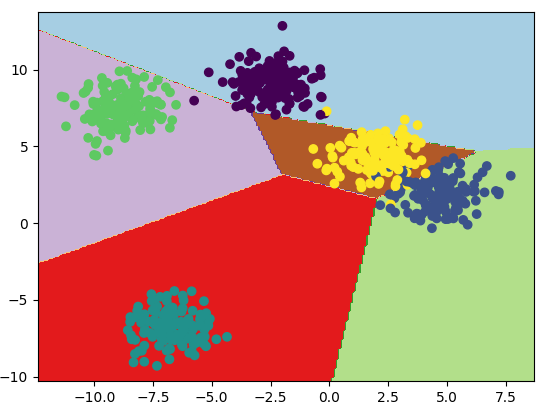
\includegraphics[width=\linewidth]{images/perceptron_train_blobs}
		\caption{Перцептрон: обучающая выборка}
	\end{subfigure}
	\begin{subfigure}{0.49\linewidth}
		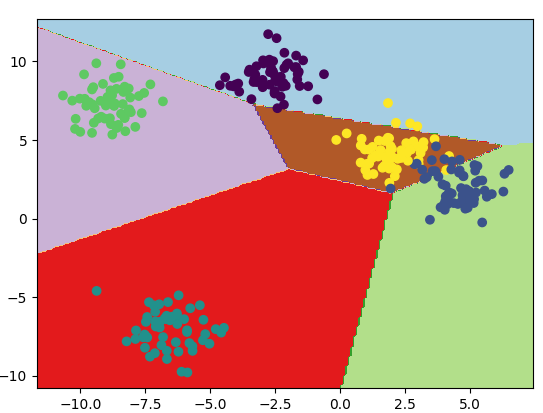
\includegraphics[width=\linewidth]{images/perceptron_test_blobs}
		\caption{Перцептрон: тестовая выборка}
	\end{subfigure}
	\begin{subfigure}{0.49\linewidth}
		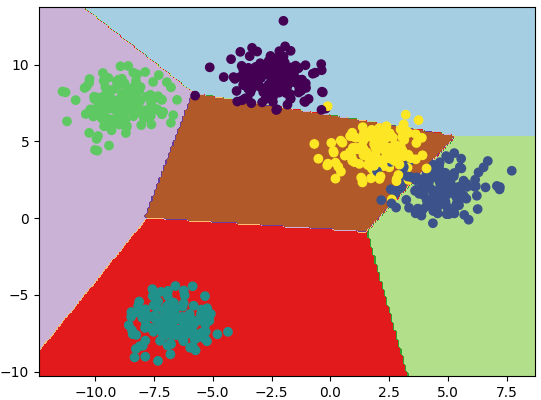
\includegraphics[width=\linewidth]{images/sgd_train_blobs}
		\caption{Линейный классификатор: обучающий набор}
	\end{subfigure}
	\begin{subfigure}{0.49\linewidth}
		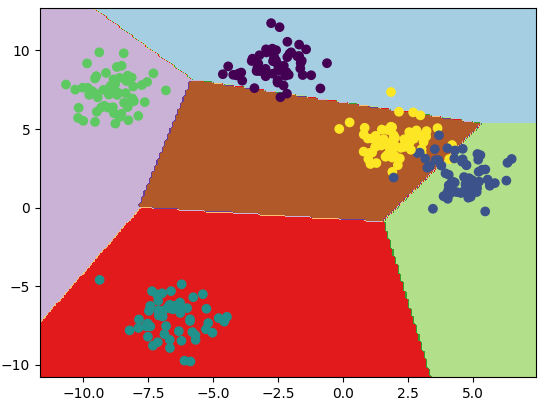
\includegraphics[width=\linewidth]{images/sgd_test_blobs}
		\caption{Линейный классификатор: тестовый набор}
	\end{subfigure}

	\caption{\textit{Decision surface} и выборки данных}
	\label{img:blobs}
\end{figure}

Метрики на тестовом множестве показаны в таблице \ref{tbl:first_blobs_metrics}.
\begin{table}[h]
	\centering
	\begin{tabular}{|c|c|c|c|c|}
		\hline
		& \textbf{accuracy} & \textbf{precision} & \textbf{recall} & \textbf{f1} \\\hline
		Perceptron    & 0.9433 & 0.9487 & 0.9458 & 0.9449 \\\hline
		SGDClassifier & 0.9500 & 0.9558 & 0.9520 & 0.9517 \\\hline
	\end{tabular}
	\caption{Метрики на тестовом множестве}
	\label{tbl:first_blobs_metrics}
\end{table}

Статистика и картинки получены следующим скриптом:\\
\noindent\fbox{%
	\parbox{\textwidth}{%
		\centering
	python3.8 code/main.py}%
}

Так как однослойный перцептрон в своей основе имеет тот же принцип, что и линейный классификатор, попробуем добиться одинаковых результатов на обеих моделях. 


\begin{table}[h]
	\centering
	\begin{tabular}{|c|c|c|c|c|}
		\hline
		& \textbf{accuracy} & \textbf{precision} & \textbf{recall} & \textbf{f1} \\\hline
		Perceptron    & 0.8167 & 0.8324 & 0.8229 & 0.8009 \\\hline
	\end{tabular}
	\caption{Перцептрону указана функция регуляризации \textit{$l_2$}}
\end{table}

Скрипт получения такого результата:

\noindent\fbox{%
	\parbox{\textwidth}{%
		\centering
	python3.8 code/main.py -{}-penalty\_perceptron l2}%
}

\begin{table}[h]
	\centering
	\begin{tabular}{|c|c|c|c|c|}
		\hline
		& \textbf{accuracy} & \textbf{precision} & \textbf{recall} & \textbf{f1} \\\hline
		Perceptron    & 0.9767 & 0.9774 & 0.9776 & 0.9774 \\\hline
	\end{tabular}
	\caption{Перцептрону добавлен флаг ранней остановки, если оценка на валидации перестаёт улучшаться}
\end{table}


Скрипт получения такого результата:

\noindent\fbox{%
	\parbox{\textwidth}{%
		\centering
	python3.8 code/main.py -{}-early\_stopping\_perceptron 1}%
}

Перцептрон с ранней остановкой перегнал по метрикам линейный классификатор из библиотеки \textbf{sklearn}. Попробуем улучшить его путём изменения входных параметров. Укажем флаг ранней остановки, который помог с перцептроном, и добавим знаки после запятой, чтобы лучше видеть картину при близости результатов:

\begin{table}[!h]
	\centering
	\begin{tabular}{|c|c|c|c|c|}
		\hline
		& \textbf{accuracy} & \textbf{precision} & \textbf{recall} & \textbf{f1} \\\hline
		Perceptron       & 0.9767 & 0.9774 & 0.9776 & 0.9774 \\\hline
		SGDClassifier    & 0.9667 & 0.9696 & 0.9682 & 0.9678 \\\hline
	\end{tabular}
	\caption{Линейному классификатору добавлен флаг ранней остановки. }
	\label{tbl:close_blobs}
\end{table}

Сейчас, судя по таблице \ref{tbl:close_blobs} разница по метрикам около одного процента.

Скрипт получения такого результата:

\noindent\fbox{%
	\parbox{\textwidth}{%
		\centering
	python3.8 code/main.py -{}-early\_stopping\_perceptron 1 -{}-early\_stopping\_sgd 1}%
}

\begin{table}[!h]
	\centering
	\begin{tabular}{|c|c|c|c|c|}
		\hline
		& \textbf{accuracy} & \textbf{precision} & \textbf{recall} & \textbf{f1} \\\hline
		Perceptron       & 0.9767 & 0.9767 & 0.9767 & 0.9767 \\\hline
		SGDClassifier    & 0.9700 & 0.9714 & 0.9713 & 0.9710 \\\hline
	\end{tabular}
	\caption{Линейному классификатору добавлен флаг ранней остановки и отключена функция регуляризации (по умолчанию включена и равна $l_2$).}
\end{table}

Это наименьшая разница в метриках, которую удалось добиться изменением параметров классов (без полного превращения линейного классификатора в перцептрон по параметрам). \textit{Decision surface} при этом получились следующие (рис. \ref{img:blobs_last}).

Скрипт получения такого результата:

\noindent\fbox{%
	\parbox{\textwidth}{%
		\centering
	python3.8 code/main.py -{}-early\_stopping\_perceptron 1 -{}-early\_stopping\_sgd 1 -{}-penalty\_sgd None}%
}

\begin{figure}[h]
	\centering
	\begin{subfigure}{0.49\linewidth}
		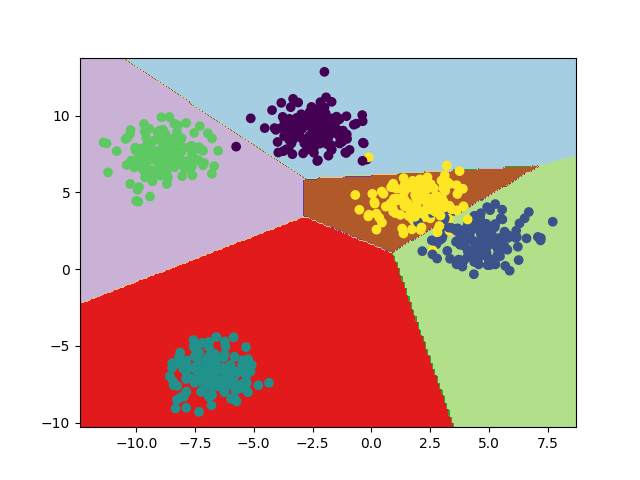
\includegraphics[width=\linewidth]{images/perceptron_train_blobs_last}
		\caption{Перцептрон: обучающая выборка}
	\end{subfigure}
	\begin{subfigure}{0.49\linewidth}
		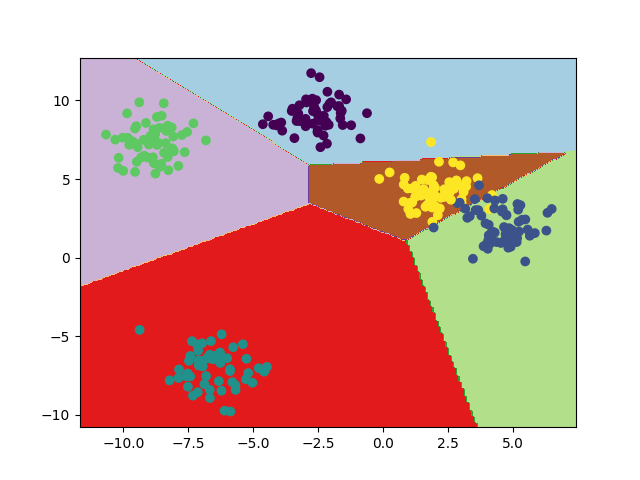
\includegraphics[width=\linewidth]{images/perceptron_test_blobs_last}
		\caption{Перцептрон: тестовая выборка}
	\end{subfigure}
	\begin{subfigure}{0.49\linewidth}
		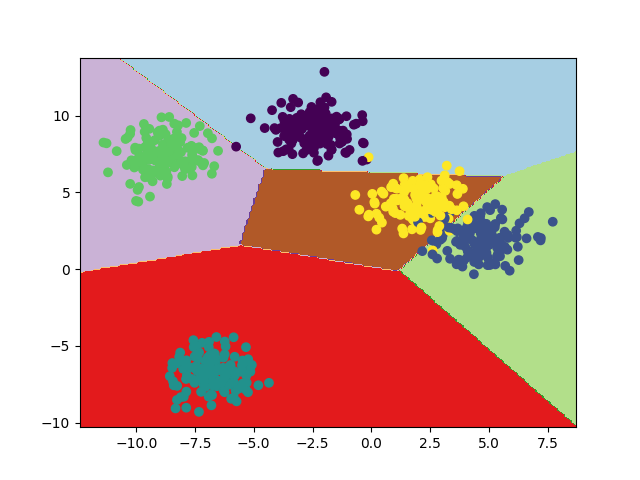
\includegraphics[width=\linewidth]{images/sgd_train_blobs_last}
		\caption{Линейный классификатор: обучающий набор}
	\end{subfigure}
	\begin{subfigure}{0.49\linewidth}
		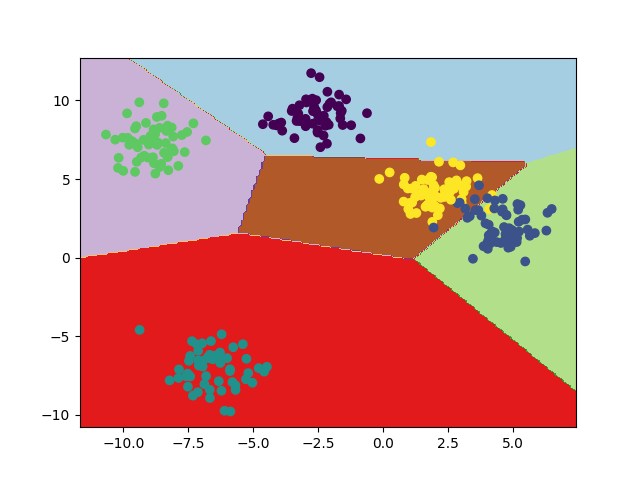
\includegraphics[width=\linewidth]{images/sgd_test_blobs_last}
		\caption{Линейный классификатор: тестовый набор}
	\end{subfigure}

	\caption{\textit{Decision surface} и выборки данных с новыми параметрами моделей}
	\label{img:blobs_last}
\end{figure}